% !TEX root = ../main.tex
\section{Execução da Suíte de Testes}

% ----------------------------------------------------------------------------
% 4.1 CONFIGURAÇÃO
% ----------------------------------------------------------------------------

\subsection{Configuração do Ambiente}

A configuração do ambiente foi realizada separadamente para cada repositório.
Inicialmente, os repositórios foram clonados 
e suas dependências foram instaladas por meio do gerenciador de pacotes npm.

No educado-api, a instalação das dependências foi realizada com \texttt{npm install}.
No educado-web, foi utilizado inicialmente o comando \texttt{npm ci}.
Entretanto, para realizar a coleta de cobertura de código, 
foi necessário instalar adicionalmente o pacote \texttt{@vitest/coverage-v8} 
e adaptar a configuração do Vitest.
No educado-app, as dependências foram instaladas com \texttt{npm install} 
e a configuração do Jest foi adaptada para permitir a coleta de cobertura de código.

As versões e principais ferramentas identificadas no ambiente utilizado são apresentadas nas Tabelas \ref{tab:ambienteApi}, \ref{tab:ambienteWeb} e \ref{tab:ambienteApp}.

Através da leitura do README de cada repositório, 
assim como análise dos seus arquivos, 
foi encontrado o uso das seguintes configurações de ambiente

\begin{table}[H]
\centering
\caption{Configuração do ambiente utilizado no educado-api.}
\label{tab:ambienteApi}
\begin{tabularx}{\textwidth}{l X X}
\toprule
\textbf{Componente} & \textbf{Versão} & \textbf{Evidência}\\
\midrule
Sistema operacional & Windows 11 Home Single Language - 25H2 & Ambiente utilizado \\
Linguagem & TypeScript 5.9.3 com Node.js 20 e npm 11.6.0 & \texttt{package.json} e \texttt{README.md} \cite{educado-repos} \\
Frameworks & Express \textasciicircum{}5.2.1 &  \texttt{package.json} \cite{educado-repos} \\
Ferramenta de build & Nixpacks para deploy &  \texttt{README.md} \cite{educado-repos}\\
Banco de dados & PostgreSQL 16 &  \texttt{README.md} \cite{educado-repos}\\
Outros & Jest \textasciicircum{}30.3.0 & \texttt{package.json} \cite{educado-repos} \\
\bottomrule
\end{tabularx}
\end{table}

\begin{table}[H]
\centering
\caption{Configuração do ambiente utilizado no educado-web.}
\label{tab:ambienteWeb}
\begin{tabularx}{\textwidth}{l X X}
\toprule
\textbf{Componente} & \textbf{Versão} & \textbf{Evidências} \\
\midrule
Sistema operacional & Windows 11 Home Single Language - 25H2 & Ambiente utilizado \\
Linguagem & TypeScript \textasciicircum{}5.9.3 com Node.js 20 e npm 11.6.0 & \texttt{package.json} e \texttt{README.md} \cite{educado-repos} \\
Frameworks & -- & \texttt{package.json} e \texttt{README.md} \cite{educado-repos} \\
Ferramenta de build & vite \textasciicircum{}7.3.5 & \texttt{package.json} e \texttt{README.md} \cite{educado-repos} \\
Banco de dados & -- & --\\
Outros & Vitest \textasciicircum{}4.1.10 & \texttt{package.json} e \texttt{README.md} \cite{educado-repos} \\
\bottomrule
\end{tabularx}
\end{table}

\begin{table}[H]
\centering
\caption{Configuração do ambiente utilizado no educado-app.}
\label{tab:ambienteApp}
\begin{tabularx}{\textwidth}{l X X}
\toprule
\textbf{Componente} & \textbf{Versão} & \textbf{Evidências} \\
\midrule
Sistema operacional & Windows 11 Home Single Language - 25H2 & Ambiente utilizado \\
Linguagem & TypeScript \textasciitilde{}6.0.3 & \texttt{package.json} e \texttt{README.md} \cite{educado-repos} \\
Frameworks &  React native 0.85.3, React 19.2.3, Expo SDK \textasciitilde{}56.0.12 e expo-router \textasciitilde{}56.2.11 & \texttt{package.json} e \texttt{README.md} \cite{educado-repos} \\
Ferramenta de build & Android SDK e EAS-cli >= 16.28.0 & \texttt{flake.nix} e \texttt{README.md} \cite{educado-repos} \\
Banco de dados & -- & -- \\
Outros & jest-expo 56.0.5 para testes & \texttt{package.json} \cite{educado-repos} \\
\bottomrule
\end{tabularx}
\end{table}


% ----------------------------------------------------------------------------
% 4.2 EXECUÇÃO
% ----------------------------------------------------------------------------

\subsection{Procedimento de Execução}

A suíte de testes foi executada separadamente em cada repositório.
Os comandos utilizados pela equipe são apresentados a seguir.

\begin{lstlisting}[language=bash]
# educado-api
cd educado-api
npm install
npm run test:coverage

# educado-web
cd educado-web
npm ci
npm install -D @vitest/coverage-v8

# Adaptacao do vitest.config.ts
npx vitest --coverage --run

# educado-app
cd educado-app
npm install

# Adaptacao da configuracao do Jest no package.json
npx jest --coverage
\end{lstlisting}

No educado-api, foi utilizado o comando \texttt{npm run test:coverage}, 
disponibilizado pelo próprio projeto para executar os testes 
e gerar o relatório de cobertura.

No educado-web, foi necessário instalar o pacote \texttt{@vitest/coverage-v8} 
e adaptar o arquivo \texttt{vitest.config.ts} para permitir a coleta de cobertura.

No educado-app, foi necessário adaptar a configuração do Jest no arquivo \texttt{package.json} para realizar a coleta de cobertura.

As alterações realizadas no educado-web e no educado-app foram feitas exclusivamente para possibilitar a medição de cobertura.

% ----------------------------------------------------------------------------
% 4.3 RESULTADOS
% ----------------------------------------------------------------------------

\subsection{Resultados da Execução}

Os resultados obtidos na execução dos testes dos três repoositórios são apresentados na tabela \ref{tab:execucao}

\begin{table}[H]
\centering
\caption{Resultado da execução da suíte de testes.}
\label{tab:execucao}
\begin{tabular}{lrrr}
\toprule
\textbf{Indicador} & \textbf{API}  & \textbf{WEB} & \textbf{APP}\\
\midrule
Testes executados & 506 & 1 & 1 \\
Testes aprovados & 506 & 1 & 1 \\
Testes falhos & 0 & 0 & 0 \\
Testes ignorados & 0 & 0 & 0 \\
Tempo de execução & 8,20 s & 2,56 s & 9,03 s \\
\bottomrule
\end{tabular}
\end{table}


% ----------------------------------------------------------------------------
% 4.4 COBERTURA
% ----------------------------------------------------------------------------

\subsection{Cobertura de Código}

A cobertura de código foi coletada por meio do Jest no educado-api 
e por meio do Vitest com o plugin \texttt{@vitest/coverage-v8} no educado-web.
No educado-app, a cobertura foi coletada utilizando o Jest configurado para o ambiente Expo.

No caso do educado-web e do educado-app, a coleta de cobertura exigiu alterações realizadas pela equipe nas configurações dos projetos.
Dessa forma, os resultados apresentados representam a cobertura observada após essas adaptações.

\begin{table}[H]
\centering
\caption{Cobertura de código.}
\label{tab:cobertura}
\begin{tabular}{lccc}
\toprule
\textbf{Métrica} & \textbf{API} & \textbf{WEB} & \textbf{APP} \\
\midrule
Linhas & 78,90\% & 0,40\%  & 0,71\% \\
Branches & 69,26\% & 0,26\% & 1,04\% \\
Métodos/Funções & 78,00\% & 0,73\% & 0,81\% \\
Statements & 79,36\% & 0,39\% & 0,72\% \\
\bottomrule
\end{tabular}
\end{table}

As evidências dos relatórios de cobertura são apresentadas nas Figuras \ref{fig:cobertura-api}, \ref{fig:cobertura-web} e \ref{fig:cobertura-app}.

\subsubsection{Comprovação da Cobertura de Código}
\begin{figure}[H]
    \centering
    \label{fig:cobertura-api}
    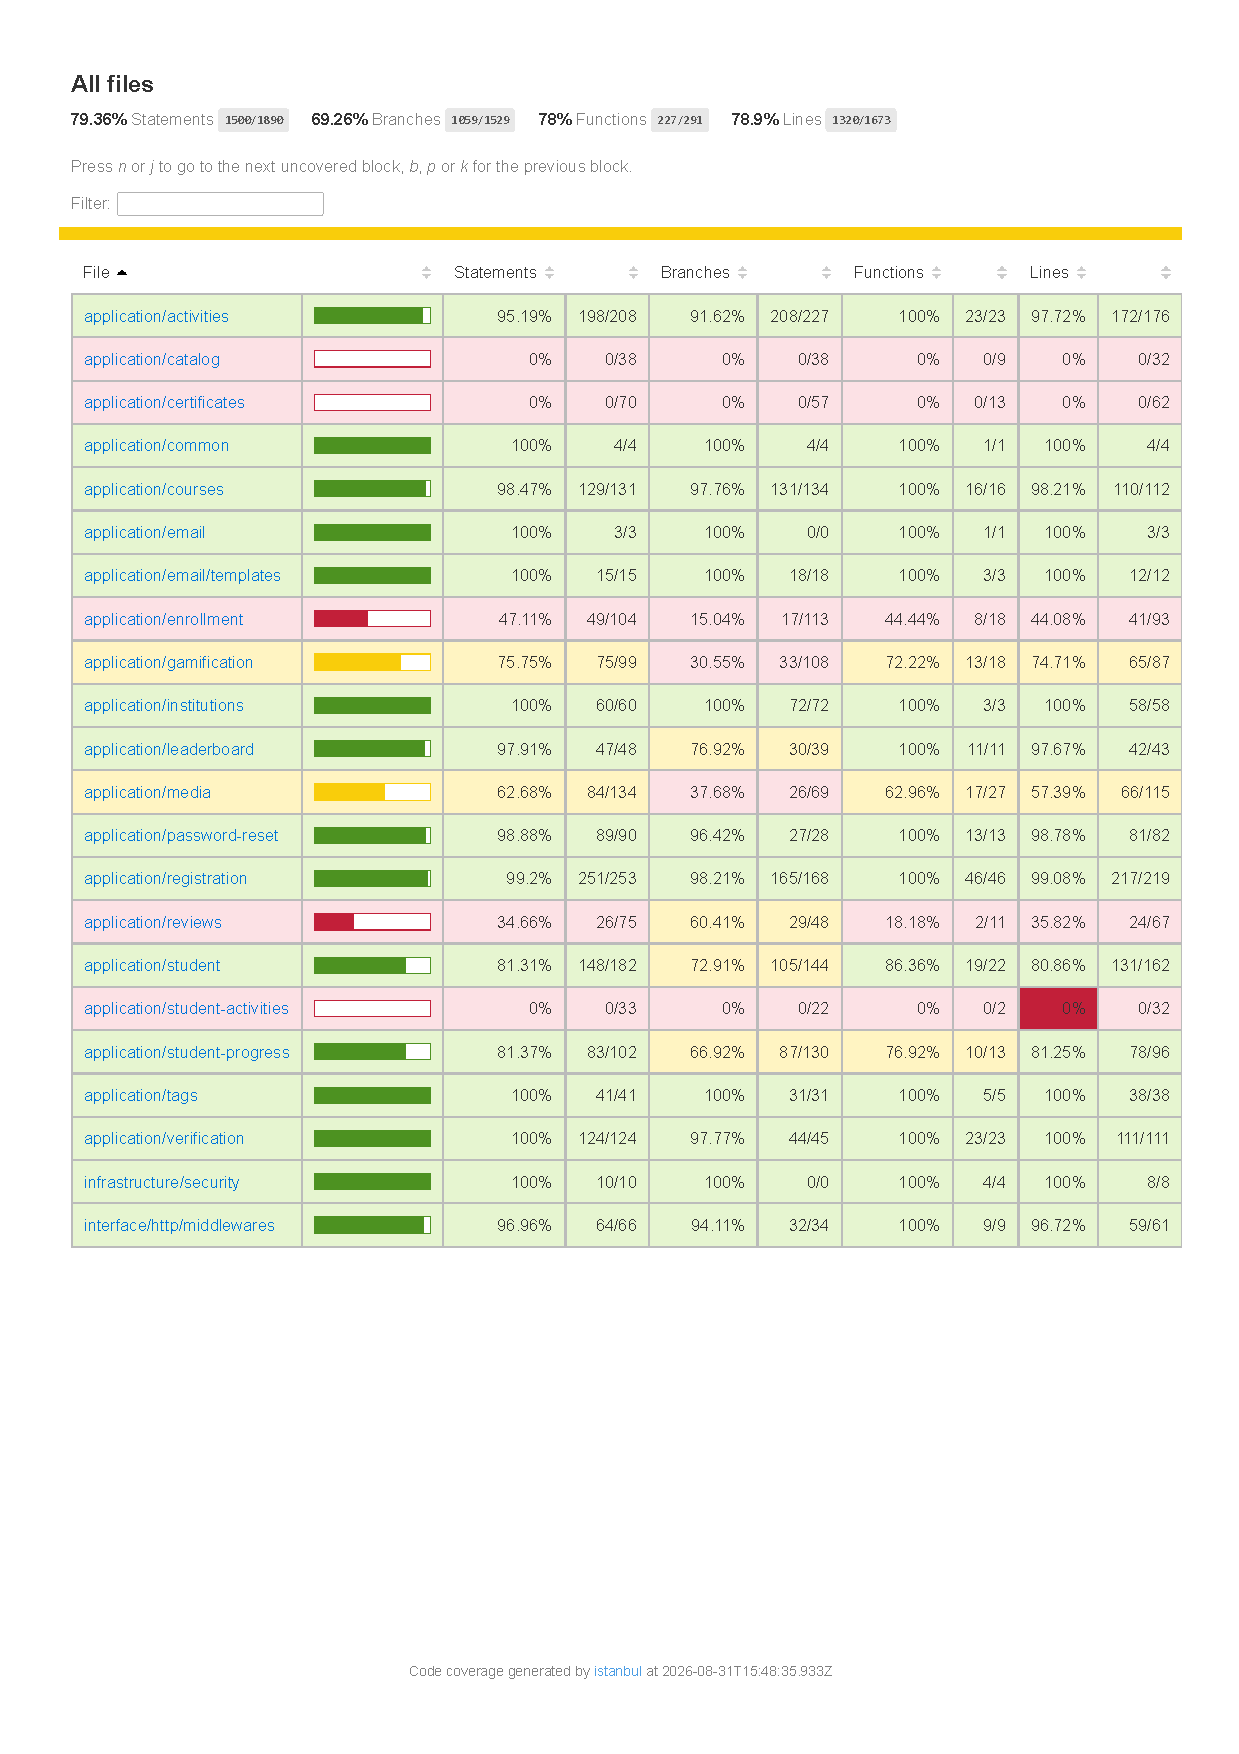
\includegraphics[width=\textwidth, trim=0 8cm 0 0,clip]{figuras/cobertura_inicial_api.pdf}
    \caption{Relatório de cobertura dos testes da API}
\end{figure}

\begin{figure}[H]
    \centering
    \label{fig:cobertura-web}
    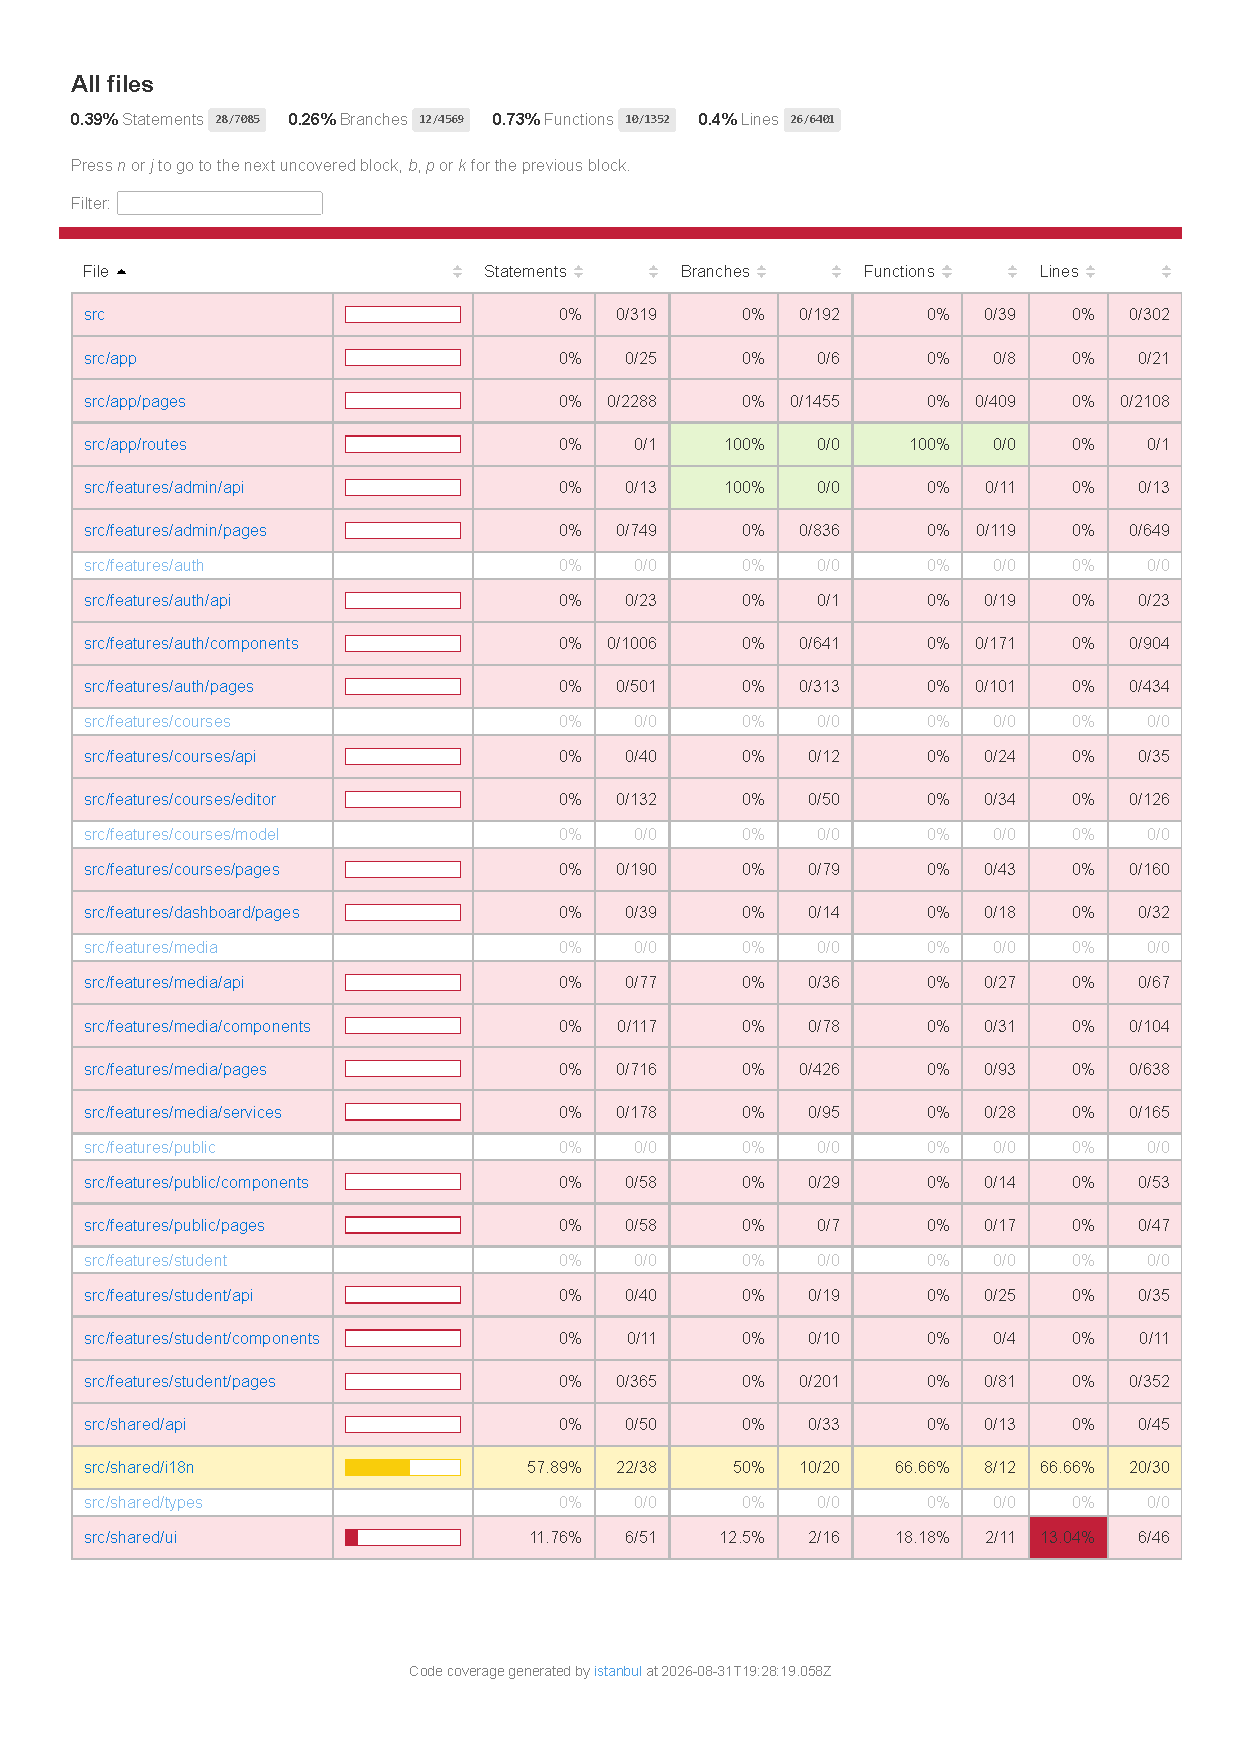
\includegraphics[width=\textwidth, trim=0 2cm 0 0,clip]{figuras/cobertura_inicial_web.pdf}
    \caption{Relatório de cobertura dos testes do Web}
\end{figure}

\begin{figure}[H]
    \centering
    \label{fig:cobertura-app}
    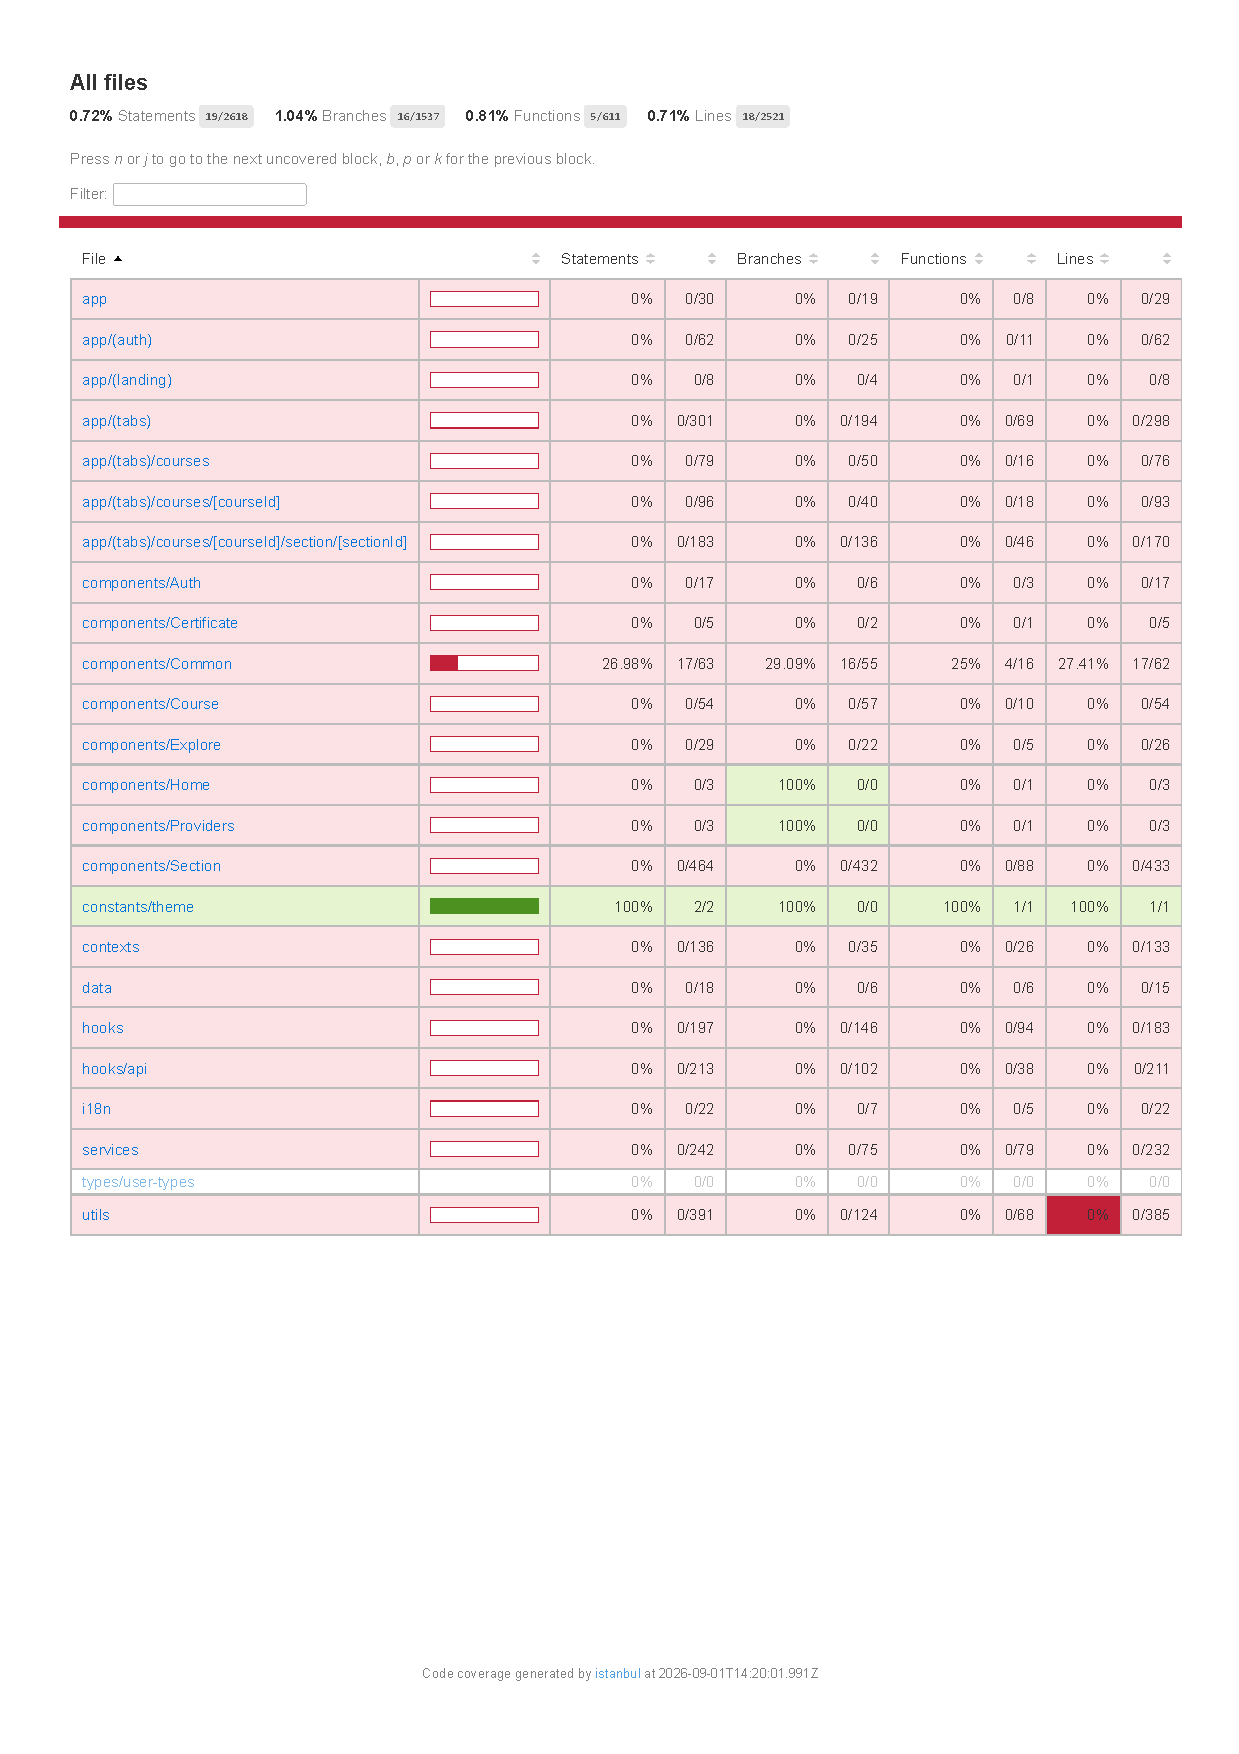
\includegraphics[width=\textwidth, trim=0 8cm 0 0,clip]{figuras/cobertura_inicial_app.pdf}
    \caption{Relatório de cobertura dos testes do app}
\end{figure}

% ----------------------------------------------------------------------------
% 4.5 PROBLEMAS
% ----------------------------------------------------------------------------

\subsection{Problemas Encontrados Durante a Execução}
\begin{itemize}
\item \textbf{Problemas de configuração:}
o educado-web e o educado-app não estavam configurados, originalmente, para apresentar a cobertura dos arquivos do projeto da mesma forma que a API.
Para possibilitar a coleta dos dados utilizados nesta análise, foram realizadas adaptações no \texttt{vitest.config.ts} do educado-web e na configuração do Jest, presente no \texttt{package.json}, do educado-app.

\item \textbf{Problemas de dependências:}
o educado-web não possuía originalmente o pacote necessário para a coleta de cobertura com Vitest.
Foi necessária a instalação do pacote \texttt{@vitest/coverage-v8} utilizando \texttt{npm install -D @vitest/coverage-v8}.

\item \textbf{Problemas relacionados ao ambiente:}
não foram identificados problemas que impedissem a execução das suítes após a configuração dos repositórios.

\item \textbf{Testes que falharam:}
nenhum teste apresentou falha durante a execução realizada pela equipe.
Foram executados 506 testes no educado-api, um no educado-web e um no educado-app, todos aprovados.

\item \textbf{Possíveis defeitos do projeto:}
a execução do comando \texttt{npm audit} identificou vulnerabilidades nas dependências dos três repositórios.

\begin{lstlisting}[language=bash]
$ cd educado-api
$ npm audit
...
11 vulnerabilities (1 low, 7 moderate, 3 high)
...

$ cd ../educado-app
$ npm audit
... 
23 vulnerabilities (17 moderate, 6 high)
... 

$ cd ../educado-web
$ npm audit
... 
1 low severity vulnerability
...
\end{lstlisting}

\end{itemize}
